% Options for packages loaded elsewhere
\PassOptionsToPackage{unicode}{hyperref}
\PassOptionsToPackage{hyphens}{url}
%
\documentclass[
]{article}
\usepackage{amsmath,amssymb}
\usepackage{lmodern}
\usepackage{ifxetex,ifluatex}
\ifnum 0\ifxetex 1\fi\ifluatex 1\fi=0 % if pdftex
  \usepackage[T1]{fontenc}
  \usepackage[utf8]{inputenc}
  \usepackage{textcomp} % provide euro and other symbols
\else % if luatex or xetex
  \usepackage{unicode-math}
  \defaultfontfeatures{Scale=MatchLowercase}
  \defaultfontfeatures[\rmfamily]{Ligatures=TeX,Scale=1}
\fi
% Use upquote if available, for straight quotes in verbatim environments
\IfFileExists{upquote.sty}{\usepackage{upquote}}{}
\IfFileExists{microtype.sty}{% use microtype if available
  \usepackage[]{microtype}
  \UseMicrotypeSet[protrusion]{basicmath} % disable protrusion for tt fonts
}{}
\makeatletter
\@ifundefined{KOMAClassName}{% if non-KOMA class
  \IfFileExists{parskip.sty}{%
    \usepackage{parskip}
  }{% else
    \setlength{\parindent}{0pt}
    \setlength{\parskip}{6pt plus 2pt minus 1pt}}
}{% if KOMA class
  \KOMAoptions{parskip=half}}
\makeatother
\usepackage{xcolor}
\IfFileExists{xurl.sty}{\usepackage{xurl}}{} % add URL line breaks if available
\IfFileExists{bookmark.sty}{\usepackage{bookmark}}{\usepackage{hyperref}}
\hypersetup{
  pdftitle={Exerciseses chapter 4},
  pdfauthor={Andreas Slåttelid},
  hidelinks,
  pdfcreator={LaTeX via pandoc}}
\urlstyle{same} % disable monospaced font for URLs
\usepackage[margin=1in]{geometry}
\usepackage{color}
\usepackage{fancyvrb}
\newcommand{\VerbBar}{|}
\newcommand{\VERB}{\Verb[commandchars=\\\{\}]}
\DefineVerbatimEnvironment{Highlighting}{Verbatim}{commandchars=\\\{\}}
% Add ',fontsize=\small' for more characters per line
\usepackage{framed}
\definecolor{shadecolor}{RGB}{248,248,248}
\newenvironment{Shaded}{\begin{snugshade}}{\end{snugshade}}
\newcommand{\AlertTok}[1]{\textcolor[rgb]{0.94,0.16,0.16}{#1}}
\newcommand{\AnnotationTok}[1]{\textcolor[rgb]{0.56,0.35,0.01}{\textbf{\textit{#1}}}}
\newcommand{\AttributeTok}[1]{\textcolor[rgb]{0.77,0.63,0.00}{#1}}
\newcommand{\BaseNTok}[1]{\textcolor[rgb]{0.00,0.00,0.81}{#1}}
\newcommand{\BuiltInTok}[1]{#1}
\newcommand{\CharTok}[1]{\textcolor[rgb]{0.31,0.60,0.02}{#1}}
\newcommand{\CommentTok}[1]{\textcolor[rgb]{0.56,0.35,0.01}{\textit{#1}}}
\newcommand{\CommentVarTok}[1]{\textcolor[rgb]{0.56,0.35,0.01}{\textbf{\textit{#1}}}}
\newcommand{\ConstantTok}[1]{\textcolor[rgb]{0.00,0.00,0.00}{#1}}
\newcommand{\ControlFlowTok}[1]{\textcolor[rgb]{0.13,0.29,0.53}{\textbf{#1}}}
\newcommand{\DataTypeTok}[1]{\textcolor[rgb]{0.13,0.29,0.53}{#1}}
\newcommand{\DecValTok}[1]{\textcolor[rgb]{0.00,0.00,0.81}{#1}}
\newcommand{\DocumentationTok}[1]{\textcolor[rgb]{0.56,0.35,0.01}{\textbf{\textit{#1}}}}
\newcommand{\ErrorTok}[1]{\textcolor[rgb]{0.64,0.00,0.00}{\textbf{#1}}}
\newcommand{\ExtensionTok}[1]{#1}
\newcommand{\FloatTok}[1]{\textcolor[rgb]{0.00,0.00,0.81}{#1}}
\newcommand{\FunctionTok}[1]{\textcolor[rgb]{0.00,0.00,0.00}{#1}}
\newcommand{\ImportTok}[1]{#1}
\newcommand{\InformationTok}[1]{\textcolor[rgb]{0.56,0.35,0.01}{\textbf{\textit{#1}}}}
\newcommand{\KeywordTok}[1]{\textcolor[rgb]{0.13,0.29,0.53}{\textbf{#1}}}
\newcommand{\NormalTok}[1]{#1}
\newcommand{\OperatorTok}[1]{\textcolor[rgb]{0.81,0.36,0.00}{\textbf{#1}}}
\newcommand{\OtherTok}[1]{\textcolor[rgb]{0.56,0.35,0.01}{#1}}
\newcommand{\PreprocessorTok}[1]{\textcolor[rgb]{0.56,0.35,0.01}{\textit{#1}}}
\newcommand{\RegionMarkerTok}[1]{#1}
\newcommand{\SpecialCharTok}[1]{\textcolor[rgb]{0.00,0.00,0.00}{#1}}
\newcommand{\SpecialStringTok}[1]{\textcolor[rgb]{0.31,0.60,0.02}{#1}}
\newcommand{\StringTok}[1]{\textcolor[rgb]{0.31,0.60,0.02}{#1}}
\newcommand{\VariableTok}[1]{\textcolor[rgb]{0.00,0.00,0.00}{#1}}
\newcommand{\VerbatimStringTok}[1]{\textcolor[rgb]{0.31,0.60,0.02}{#1}}
\newcommand{\WarningTok}[1]{\textcolor[rgb]{0.56,0.35,0.01}{\textbf{\textit{#1}}}}
\usepackage{graphicx}
\makeatletter
\def\maxwidth{\ifdim\Gin@nat@width>\linewidth\linewidth\else\Gin@nat@width\fi}
\def\maxheight{\ifdim\Gin@nat@height>\textheight\textheight\else\Gin@nat@height\fi}
\makeatother
% Scale images if necessary, so that they will not overflow the page
% margins by default, and it is still possible to overwrite the defaults
% using explicit options in \includegraphics[width, height, ...]{}
\setkeys{Gin}{width=\maxwidth,height=\maxheight,keepaspectratio}
% Set default figure placement to htbp
\makeatletter
\def\fps@figure{htbp}
\makeatother
\setlength{\emergencystretch}{3em} % prevent overfull lines
\providecommand{\tightlist}{%
  \setlength{\itemsep}{0pt}\setlength{\parskip}{0pt}}
\setcounter{secnumdepth}{-\maxdimen} % remove section numbering
\ifluatex
  \usepackage{selnolig}  % disable illegal ligatures
\fi

\title{Exerciseses chapter 4}
\author{Andreas Slåttelid}
\date{23/2/2022}

\begin{document}
\maketitle

\hypertarget{exercise-4.3}{%
\subsection{Exercise 4.3}\label{exercise-4.3}}

In this exercise we are considering a disability insurance, hence
\(S = \{*,\diamond ,\dagger \}\). The contractual information given are:
as follows:

\begin{Shaded}
\begin{Highlighting}[]
\NormalTok{x }\OtherTok{\textless{}{-}} \DecValTok{30}     \CommentTok{\#age}
\NormalTok{T }\OtherTok{\textless{}{-}} \DecValTok{35}     \CommentTok{\#length of contract}
\NormalTok{D }\OtherTok{\textless{}{-}} \DecValTok{20000}  \CommentTok{\#disability pension}
\NormalTok{r }\OtherTok{\textless{}{-}} \FloatTok{0.03}   \CommentTok{\#intereset rate}
\NormalTok{premium\_yearly }\OtherTok{\textless{}{-}} \DecValTok{2500}
\end{Highlighting}
\end{Shaded}

Furthermore the transition rates are given by:

\begin{Shaded}
\begin{Highlighting}[]
\NormalTok{lambda }\OtherTok{\textless{}{-}} \ControlFlowTok{function}\NormalTok{(t)\{}
  \CommentTok{\#we do not have any t{-}dependency}
\NormalTok{  m12 }\OtherTok{\textless{}{-}} \FloatTok{0.0279} 
\NormalTok{  m13 }\OtherTok{\textless{}{-}} \FloatTok{0.0229}
\NormalTok{  m11 }\OtherTok{\textless{}{-}} \SpecialCharTok{{-}}\NormalTok{(m12}\SpecialCharTok{+}\NormalTok{m13)}
\NormalTok{  m21 }\OtherTok{\textless{}{-}} \DecValTok{0}
\NormalTok{  m23 }\OtherTok{\textless{}{-}} \FloatTok{0.0229}
\NormalTok{  m22 }\OtherTok{\textless{}{-}} \SpecialCharTok{{-}}\NormalTok{(m21}\SpecialCharTok{+}\NormalTok{m23)}
\NormalTok{  m31 }\OtherTok{\textless{}{-}}\NormalTok{ m32 }\OtherTok{\textless{}{-}}\NormalTok{ m33 }\OtherTok{\textless{}{-}} \DecValTok{0}
\NormalTok{  L }\OtherTok{\textless{}{-}} \FunctionTok{matrix}\NormalTok{(}\FunctionTok{c}\NormalTok{(m11,m12,m13,m21,m22,m23,m31,m32,m33), }\AttributeTok{nrow=}\DecValTok{3}\NormalTok{, }\AttributeTok{byrow=}\ConstantTok{TRUE}\NormalTok{)}
  
  \FunctionTok{return}\NormalTok{(L)}
\NormalTok{\}}
\end{Highlighting}
\end{Shaded}

We also have the following policy-functions: \[\begin{aligned}
a_{*}(t) &= \begin{cases}
0, &t<0 \\
-\pi t, &t\in[0,T) \\ 
-\pi T, &t\geq T
\end{cases} \\ 
a_{\diamond}(t) &= \begin{cases}
0, &t<0 \\
Dt, &t\in[0,T) \\ 
DT, &t\geq T
\end{cases} 
\end{aligned}\]

We were asked to calculate \(V_{j}^{+}(t,A)\) for \(j = *, \diamond\)
and for \(t=30\). We then get: \[\begin{aligned}
V_{*}^{+}(t,A) &= \frac{1}{v(t)}\left[\int_{t}^{T}v(s)p_{**}(x+t,x+s)da_{*}(s)   
+ \int_{t}^{T}v(s)p_{*\diamond}(x+t,x+s)da_{\diamond}(s) 
\right] \\ 
&= \frac{1}{v(t)}\left[-\pi\int_{t}^{T}v(s)p_{**}(x+t,x+s)ds   
+ D\int_{t}^{T}v(s)p_{*\diamond}(x+t,x+s)ds 
\right]
\end{aligned}\]

\newpage

\[\begin{aligned}
V_{\diamond}^{+}(t,A) &= \frac{1}{v(t)}\left[
\int_{t}^{T}v(s)p_{\diamond \diamond}(x+t, x+s)da_{\diamond}(s)
\right] \\ 
&= \frac{1}{v(t)}\left[D
\int_{t}^{T}v(s)p_{\diamond \diamond}(x+t, x+s)ds
\right] 
\end{aligned}\] We will now use an Euler-scheme to simulate what's going
on, and then use a Riemann-sum to compute the integrals: \[
\int_{a}^{b}f(x)dx \approx \sum_{i=0}^{n-1}f(x_{i}^{*})\Delta x
\] Where \(\Delta x = \frac{b-a}{n}\), which in our case corresponds to:
\(h\) and \(x_{i}^{*} \in [x_{i},x_{i+1}]\)

\begin{Shaded}
\begin{Highlighting}[]
\NormalTok{field }\OtherTok{\textless{}{-}} \ControlFlowTok{function}\NormalTok{(t,M)\{}
  \FunctionTok{return}\NormalTok{(M}\SpecialCharTok{\%*\%}\FunctionTok{lambda}\NormalTok{(t))}
\NormalTok{\}}

\CommentTok{\#field(t0, P0)}

\NormalTok{Euler }\OtherTok{\textless{}{-}} \ControlFlowTok{function}\NormalTok{(t0,P0,h,tn)\{}
  \ControlFlowTok{if}\NormalTok{(t0}\SpecialCharTok{==}\NormalTok{tn)\{ }\FunctionTok{return}\NormalTok{(P0)\}}
\NormalTok{  N }\OtherTok{\textless{}{-}}\NormalTok{ (tn}\SpecialCharTok{{-}}\NormalTok{t0)}\SpecialCharTok{/}\NormalTok{h}
\NormalTok{  D }\OtherTok{\textless{}{-}} \FunctionTok{dim}\NormalTok{(P0)[}\DecValTok{1}\NormalTok{] }\CommentTok{\#gives dimension of mxn matrix dim = c(m,n)}
  \CommentTok{\#Initial condition at s}
\NormalTok{  P }\OtherTok{\textless{}{-}} \FunctionTok{array}\NormalTok{(}\FunctionTok{diag}\NormalTok{(D}\SpecialCharTok{*}\NormalTok{(N}\SpecialCharTok{+}\DecValTok{1}\NormalTok{)), }\AttributeTok{dim=}\FunctionTok{c}\NormalTok{(D,D,N}\SpecialCharTok{+}\DecValTok{1}\NormalTok{))}
  \CommentTok{\#First iteration}
\NormalTok{  P[,,}\DecValTok{1}\NormalTok{] }\OtherTok{\textless{}{-}}\NormalTok{ P0}
  
  
  \ControlFlowTok{for}\NormalTok{(n }\ControlFlowTok{in} \DecValTok{1}\SpecialCharTok{:}\NormalTok{N)\{}
\NormalTok{    P[,,n}\SpecialCharTok{+}\DecValTok{1}\NormalTok{] }\OtherTok{\textless{}{-}}\NormalTok{ P[,,n]}\SpecialCharTok{+}\NormalTok{h}\SpecialCharTok{*}\FunctionTok{field}\NormalTok{(t0}\SpecialCharTok{+}\NormalTok{n}\SpecialCharTok{*}\NormalTok{h,P[,,n])}
\NormalTok{  \}}
  \FunctionTok{return}\NormalTok{(P) }\CommentTok{\#returns array, array(data , dim= c(3,3,2)), this stores 2 3x3 matricies}
\NormalTok{\}}

\NormalTok{t0 }\OtherTok{\textless{}{-}} \DecValTok{60}       \CommentTok{\#start age}
\NormalTok{P0 }\OtherTok{\textless{}{-}} \FunctionTok{diag}\NormalTok{(}\DecValTok{3}\NormalTok{)  }\CommentTok{\#initial start with P(s,s) = I}
\NormalTok{tn }\OtherTok{\textless{}{-}} \DecValTok{110}      \CommentTok{\#end age}
\NormalTok{h }\OtherTok{\textless{}{-}} \DecValTok{1}\SpecialCharTok{/}\DecValTok{12}      \CommentTok{\#step size }
\NormalTok{N }\OtherTok{\textless{}{-}}\NormalTok{ (tn}\SpecialCharTok{{-}}\NormalTok{t0)}\SpecialCharTok{/}\NormalTok{h }\CommentTok{\#number of steps}

\NormalTok{sol }\OtherTok{\textless{}{-}} \FunctionTok{Euler}\NormalTok{(t0,P0,h,tn) }\CommentTok{\#contains ages transition probs from 60 to 65.}

\NormalTok{v }\OtherTok{\textless{}{-}} \ControlFlowTok{function}\NormalTok{(t)\{}
  \FunctionTok{return}\NormalTok{(}\FunctionTok{exp}\NormalTok{(}\SpecialCharTok{{-}}\NormalTok{r}\SpecialCharTok{*}\NormalTok{t))}
\NormalTok{\}}


\CommentTok{\#v(s), but s in [30,35]}
\NormalTok{v\_ages }\OtherTok{\textless{}{-}} \FunctionTok{sapply}\NormalTok{(}\FunctionTok{seq}\NormalTok{(}\DecValTok{30}\NormalTok{, }\DecValTok{35}\NormalTok{, }\AttributeTok{by =}\NormalTok{ h), v) }\CommentTok{\#we apply the function v to each element}




\CommentTok{\#sum1 where we do not care about the premium until afterwards, we use Riemann{-}sum.}
\NormalTok{s1 }\OtherTok{\textless{}{-}} \DecValTok{0} 
\ControlFlowTok{for}\NormalTok{ (i }\ControlFlowTok{in} \DecValTok{1}\SpecialCharTok{:}\NormalTok{(}\FunctionTok{length}\NormalTok{(v\_ages)}\SpecialCharTok{{-}}\DecValTok{1}\NormalTok{))\{}
\NormalTok{  s1 }\OtherTok{\textless{}{-}}\NormalTok{ s1 }\SpecialCharTok{+}\NormalTok{ v\_ages[i]}\SpecialCharTok{*}\NormalTok{sol[}\DecValTok{1}\NormalTok{,}\DecValTok{1}\NormalTok{, ][i]}\SpecialCharTok{*}\NormalTok{h }\CommentTok{\#survival i.e * {-}\textgreater{} *}
\NormalTok{\}}

\CommentTok{\#sum2: do not care about D=20.000 until afterwards}
\NormalTok{s2 }\OtherTok{\textless{}{-}} \DecValTok{0} 
\ControlFlowTok{for}\NormalTok{ (i }\ControlFlowTok{in} \DecValTok{1}\SpecialCharTok{:}\NormalTok{(}\FunctionTok{length}\NormalTok{(v\_ages)}\SpecialCharTok{{-}}\DecValTok{1}\NormalTok{))\{}
\NormalTok{  s2 }\OtherTok{\textless{}{-}}\NormalTok{ s2 }\SpecialCharTok{+}\NormalTok{ v\_ages[i]}\SpecialCharTok{*}\NormalTok{sol[}\DecValTok{1}\NormalTok{,}\DecValTok{2}\NormalTok{,][i]}\SpecialCharTok{*}\NormalTok{h }\CommentTok{\#disability i.e * {-}\textgreater{} dis}
\NormalTok{\}}
 
\CommentTok{\#V*(30, A): }
\NormalTok{V\_30\_A }\OtherTok{\textless{}{-}}\NormalTok{ (}\DecValTok{1}\SpecialCharTok{/}\FunctionTok{v}\NormalTok{(}\DecValTok{30}\NormalTok{))}\SpecialCharTok{*}\NormalTok{((}\SpecialCharTok{{-}}\DecValTok{1}\NormalTok{)}\SpecialCharTok{*}\NormalTok{premium\_yearly}\SpecialCharTok{*}\NormalTok{s1 }\SpecialCharTok{+}\NormalTok{ D}\SpecialCharTok{*}\NormalTok{s2)}
\NormalTok{V\_30\_A}
\end{Highlighting}
\end{Shaded}

\begin{verbatim}
## [1] -4781.495
\end{verbatim}

\begin{Shaded}
\begin{Highlighting}[]
\CommentTok{\#V\_[disabeld](30,A): }

\NormalTok{s3 }\OtherTok{\textless{}{-}} \DecValTok{0} 
\ControlFlowTok{for}\NormalTok{ (i }\ControlFlowTok{in} \DecValTok{1}\SpecialCharTok{:}\NormalTok{(}\FunctionTok{length}\NormalTok{(v\_ages)}\SpecialCharTok{{-}}\DecValTok{1}\NormalTok{))\{}
\NormalTok{  s3 }\OtherTok{\textless{}{-}}\NormalTok{ s3 }\SpecialCharTok{+}\NormalTok{ v\_ages[i]}\SpecialCharTok{*}\NormalTok{sol[}\DecValTok{2}\NormalTok{,}\DecValTok{2}\NormalTok{,][i]}\SpecialCharTok{*}\NormalTok{h }\CommentTok{\#disability i.e dis {-}\textgreater{} dis}
\NormalTok{\}}


\CommentTok{\#V\_[disabeld](30,A): }
\NormalTok{V\_30\_dis }\OtherTok{\textless{}{-}}\NormalTok{ (}\DecValTok{1}\SpecialCharTok{/}\FunctionTok{v}\NormalTok{(}\DecValTok{30}\NormalTok{))}\SpecialCharTok{*}\NormalTok{D}\SpecialCharTok{*}\NormalTok{s3}
\NormalTok{V\_30\_dis}
\end{Highlighting}
\end{Shaded}

\begin{verbatim}
## [1] 88057.1
\end{verbatim}

\newpage

\hypertarget{exercise-4.6}{%
\subsection{Exercise 4.6}\label{exercise-4.6}}

Required-libraries

\begin{Shaded}
\begin{Highlighting}[]
\NormalTok{list.of.packages }\OtherTok{\textless{}{-}} \FunctionTok{c}\NormalTok{(}\StringTok{"tidyverse"}\NormalTok{, }\StringTok{"scales"}\NormalTok{)}
\NormalTok{new.packages }\OtherTok{\textless{}{-}}\NormalTok{ list.of.packages[}\SpecialCharTok{!}\NormalTok{(list.of.packages }\SpecialCharTok{\%in\%} \FunctionTok{installed.packages}\NormalTok{()[,}\StringTok{"Package"}\NormalTok{])]}
\ControlFlowTok{if}\NormalTok{(}\FunctionTok{length}\NormalTok{(new.packages)) }\FunctionTok{install.packages}\NormalTok{(new.packages)}
\FunctionTok{library}\NormalTok{(tidyverse)}
\FunctionTok{library}\NormalTok{(scales)   }\CommentTok{\#nice formatting of plots}
\end{Highlighting}
\end{Shaded}

We are dealing with an endownment policy, in discrete time, this means
that \(S = \{*, \dagger\}\), the contractual information provided is:

\begin{Shaded}
\begin{Highlighting}[]
\NormalTok{x }\OtherTok{\textless{}{-}} \DecValTok{35}     \CommentTok{\#age}
\NormalTok{T }\OtherTok{\textless{}{-}} \DecValTok{25}     \CommentTok{\#length of contract}
\NormalTok{r }\OtherTok{\textless{}{-}} \FloatTok{0.035}  \CommentTok{\#interest rate }
\NormalTok{E }\OtherTok{\textless{}{-}} \DecValTok{125000} \CommentTok{\#endownment }
\NormalTok{B }\OtherTok{\textless{}{-}} \DecValTok{250000} \CommentTok{\#death{-}benfit}
\end{Highlighting}
\end{Shaded}

futhermore the force of mortality is given by:

\begin{Shaded}
\begin{Highlighting}[]
\NormalTok{mu }\OtherTok{\textless{}{-}} \ControlFlowTok{function}\NormalTok{(t)\{}
  \FunctionTok{return}\NormalTok{(}\FloatTok{0.0015} \SpecialCharTok{+} \FloatTok{0.0004}\SpecialCharTok{*}\NormalTok{(t}\DecValTok{{-}35}\NormalTok{))}
\NormalTok{\}}
\end{Highlighting}
\end{Shaded}

discount-factor:

\begin{Shaded}
\begin{Highlighting}[]
\NormalTok{v }\OtherTok{\textless{}{-}} \ControlFlowTok{function}\NormalTok{(t)\{}
  \FunctionTok{return}\NormalTok{(}\FunctionTok{exp}\NormalTok{(}\SpecialCharTok{{-}}\NormalTok{r}\SpecialCharTok{*}\NormalTok{t))}
\NormalTok{\}}
\end{Highlighting}
\end{Shaded}

We can also calulate the survival probability: \[\begin{aligned}
p_{**}(s,t) &= \exp\left(-\int_{s}^{t}\mu_{*\dagger}(u)du\right)
\end{aligned}\]

\begin{Shaded}
\begin{Highlighting}[]
\NormalTok{p\_surv }\OtherTok{\textless{}{-}} \ControlFlowTok{function}\NormalTok{(s,t)\{}
\NormalTok{  integral }\OtherTok{\textless{}{-}} \FloatTok{0.0015}\SpecialCharTok{*}\NormalTok{(t}\SpecialCharTok{{-}}\NormalTok{s) }\SpecialCharTok{+} \FloatTok{0.0004}\SpecialCharTok{*}\NormalTok{((}\DecValTok{1}\SpecialCharTok{/}\DecValTok{2}\NormalTok{)}\SpecialCharTok{*}\NormalTok{(t}\SpecialCharTok{\^{}}\DecValTok{2} \SpecialCharTok{{-}}\NormalTok{s}\SpecialCharTok{\^{}}\DecValTok{2}\NormalTok{) }\SpecialCharTok{+} \DecValTok{35}\SpecialCharTok{*}\NormalTok{(s}\SpecialCharTok{{-}}\NormalTok{t))}
  \FunctionTok{return}\NormalTok{(}\FunctionTok{exp}\NormalTok{(}\SpecialCharTok{{-}}\NormalTok{integral))}
\NormalTok{\}}
\FunctionTok{p\_surv}\NormalTok{(}\DecValTok{35}\NormalTok{,}\DecValTok{36}\NormalTok{)}
\end{Highlighting}
\end{Shaded}

\begin{verbatim}
## [1] 0.9983014
\end{verbatim}

We are asked to calculate the yearly premium \(\pi\), but first we start
by defining the policy functions specified in the contract.

\[\begin{aligned}
a_{*}^{Pre}(n) &= \begin{cases}
-\pi &, n = 0, \dots, T-1 \\ 
E&, n=T
\end{cases}
\;\;\;
a_{*\dagger}^{Post}(n) &= \begin{cases}
B &, n = 0, \dots, T-1 \\ 
0&, else
\end{cases}
\end{aligned}\]

We can now start to calculate the reserves, but we must be aware of what
happens at \(n = T\):

\[\begin{aligned}
V_{*}^{+}(t,A) &= \frac{1}{v(t)}\left[
\sum_{n=t}^{T}v(n)p_{**}(x+t,x+n)a_{*}^{Pre}(n) 
+ \sum_{n=t}^{T-1}v(n+1)p_{**}(x+t, x+n)p_{*\dagger}(x+n, x+n+1)a_{*\dagger}^{Post}(n)
\right] \\ 
&= \frac{1}{v(t)}\left[\alpha + \beta \right]
\end{aligned}\]

Here \(\alpha\) corresponds to the first sum, and \(\beta\) corresponds
to the second sum: \[\begin{aligned}
\alpha &= \sum_{n=t}^{T-1}v(n)p_{**}(x+t, x+n)(-\pi) + v(T)p_{**}(x+t, x+T)E \\ 
\beta &= \sum_{n=t}^{T-1}v(n+1)p_{**}(x+t, x+n)p_{*\dagger}(x+n, x+n+1)B
\end{aligned}\]

We will now use the equivalence principle, which states that the fair
premium \(\pi\) should be such that \(V_{*}(0,A) = 0\), and using this
method we end up with: \[\begin{aligned}
\pi &= \frac{v(T)p_{**}(x,x+T)E + B\sum_{n=0}^{T-1}v(n+1)p_{**}(x,x+n)p_{*\dagger}(x+n,x+n+1)}{\sum_{n=0}^{T-1}v(n)p_{**}(x,x+n)}
\end{aligned}\]

\begin{Shaded}
\begin{Highlighting}[]
\NormalTok{res1 }\OtherTok{\textless{}{-}} \DecValTok{0} 
\ControlFlowTok{for}\NormalTok{ (n }\ControlFlowTok{in} \DecValTok{0}\SpecialCharTok{:}\NormalTok{(T}\DecValTok{{-}1}\NormalTok{))\{}
\NormalTok{  res1 }\OtherTok{\textless{}{-}}\NormalTok{ res1 }\SpecialCharTok{+} \FunctionTok{v}\NormalTok{(n}\SpecialCharTok{+}\DecValTok{1}\NormalTok{)}\SpecialCharTok{*}\FunctionTok{p\_surv}\NormalTok{(x, x}\SpecialCharTok{+}\NormalTok{n)}\SpecialCharTok{*}\NormalTok{(}\DecValTok{1}\SpecialCharTok{{-}}\FunctionTok{p\_surv}\NormalTok{(x}\SpecialCharTok{+}\NormalTok{n, x}\SpecialCharTok{+}\NormalTok{n}\SpecialCharTok{+}\DecValTok{1}\NormalTok{))}
\NormalTok{\}}

\NormalTok{res2 }\OtherTok{\textless{}{-}} \DecValTok{0} 
\ControlFlowTok{for}\NormalTok{ (n }\ControlFlowTok{in} \DecValTok{0}\SpecialCharTok{:}\NormalTok{(T}\DecValTok{{-}1}\NormalTok{))\{}
\NormalTok{  res2 }\OtherTok{\textless{}{-}}\NormalTok{ res2 }\SpecialCharTok{+} \FunctionTok{v}\NormalTok{(n)}\SpecialCharTok{*}\FunctionTok{p\_surv}\NormalTok{(x, x}\SpecialCharTok{+}\NormalTok{n)}
\NormalTok{\}}

\NormalTok{above }\OtherTok{\textless{}{-}}\NormalTok{ B}\SpecialCharTok{*}\NormalTok{res1 }\SpecialCharTok{+} \FunctionTok{v}\NormalTok{(T)}\SpecialCharTok{*}\FunctionTok{p\_surv}\NormalTok{(x,x}\SpecialCharTok{+}\NormalTok{T)}\SpecialCharTok{*}\NormalTok{E }\CommentTok{\#whats above in the premium expression}
\NormalTok{below }\OtherTok{\textless{}{-}}\NormalTok{ res2            }\CommentTok{\#whats below in the premium expression}

\NormalTok{premium\_yearly }\OtherTok{\textless{}{-}}\NormalTok{ above}\SpecialCharTok{/}\NormalTok{below}
\NormalTok{premium\_yearly}
\end{Highlighting}
\end{Shaded}

\begin{verbatim}
## [1] 4095.413
\end{verbatim}

We now also want the prospective reserves: i.e \(V_{*}^{+}(t,A)\) for
\(t = 0, \dots , T\):

\begin{Shaded}
\begin{Highlighting}[]
\CommentTok{\#Present value of reserve when including premiums. }
\NormalTok{V\_reserve\_1 }\OtherTok{\textless{}{-}} \ControlFlowTok{function}\NormalTok{(}\AttributeTok{x=}\DecValTok{35}\NormalTok{, }\AttributeTok{E =} \DecValTok{125000}\NormalTok{ , }\AttributeTok{T=}\DecValTok{25}\NormalTok{)\{}
  \CommentTok{\#x: age of insured}
  \CommentTok{\#B: benefit specified in contract}
  \CommentTok{\#T: length of contract }
  
\NormalTok{  V\_star\_pre }\OtherTok{\textless{}{-}} \ConstantTok{NULL}
  \ControlFlowTok{for}\NormalTok{ (t }\ControlFlowTok{in} \DecValTok{0}\SpecialCharTok{:}\NormalTok{(T}\DecValTok{{-}1}\NormalTok{))\{}
\NormalTok{    s }\OtherTok{\textless{}{-}} \DecValTok{0} 
    \ControlFlowTok{for}\NormalTok{ (n }\ControlFlowTok{in}\NormalTok{ t}\SpecialCharTok{:}\NormalTok{(T}\DecValTok{{-}1}\NormalTok{))\{}
\NormalTok{      s }\OtherTok{\textless{}{-}}\NormalTok{ s }\SpecialCharTok{+}\NormalTok{ (}\DecValTok{1}\SpecialCharTok{/}\FunctionTok{v}\NormalTok{(t))}\SpecialCharTok{*}\NormalTok{(}\SpecialCharTok{{-}}\DecValTok{1}\NormalTok{)}\SpecialCharTok{*}\NormalTok{premium\_yearly}\SpecialCharTok{*}\FunctionTok{v}\NormalTok{(n)}\SpecialCharTok{*}\FunctionTok{p\_surv}\NormalTok{(t}\SpecialCharTok{+}\NormalTok{x, n}\SpecialCharTok{+}\NormalTok{x)}
\NormalTok{    \}}
\NormalTok{    V\_star\_pre[t}\SpecialCharTok{+}\DecValTok{1}\NormalTok{] }\OtherTok{\textless{}{-}}\NormalTok{ s  }\SpecialCharTok{+}\NormalTok{ (}\DecValTok{1}\SpecialCharTok{/}\FunctionTok{v}\NormalTok{(t))}\SpecialCharTok{*}\FunctionTok{v}\NormalTok{(T)}\SpecialCharTok{*}\FunctionTok{p\_surv}\NormalTok{(x}\SpecialCharTok{+}\NormalTok{t, x}\SpecialCharTok{+}\NormalTok{T)}\SpecialCharTok{*}\NormalTok{E }
\NormalTok{  \}}
\NormalTok{  V\_star\_pre[T}\SpecialCharTok{+}\DecValTok{1}\NormalTok{] }\OtherTok{\textless{}{-}}\NormalTok{ E }\CommentTok{\#specified by contract }
  \FunctionTok{return}\NormalTok{(V\_star\_pre)}
\NormalTok{\} }
\end{Highlighting}
\end{Shaded}

\newpage

\begin{Shaded}
\begin{Highlighting}[]
\NormalTok{V\_reserve\_2 }\OtherTok{\textless{}{-}} \ControlFlowTok{function}\NormalTok{(}\AttributeTok{x=}\DecValTok{35}\NormalTok{, }\AttributeTok{B=}\DecValTok{250000}\NormalTok{, }\AttributeTok{T=}\DecValTok{25}\NormalTok{)\{}
  \CommentTok{\#x: age of insured}
  \CommentTok{\#B: benefit specified in contract}
  \CommentTok{\#T: length of contract }
  
\NormalTok{  V\_star\_post }\OtherTok{\textless{}{-}} \ConstantTok{NULL}
  \ControlFlowTok{for}\NormalTok{ (t }\ControlFlowTok{in} \DecValTok{0}\SpecialCharTok{:}\NormalTok{(T}\DecValTok{{-}1}\NormalTok{))\{}
\NormalTok{    s }\OtherTok{\textless{}{-}} \DecValTok{0} 
    \ControlFlowTok{for}\NormalTok{ (n }\ControlFlowTok{in}\NormalTok{ t}\SpecialCharTok{:}\NormalTok{(T}\DecValTok{{-}1}\NormalTok{))\{}
\NormalTok{      s }\OtherTok{\textless{}{-}}\NormalTok{ s }\SpecialCharTok{+}\NormalTok{ (}\DecValTok{1}\SpecialCharTok{/}\FunctionTok{v}\NormalTok{(t))}\SpecialCharTok{*}\NormalTok{B}\SpecialCharTok{*}\FunctionTok{v}\NormalTok{(n}\SpecialCharTok{+}\DecValTok{1}\NormalTok{)}\SpecialCharTok{*}\FunctionTok{p\_surv}\NormalTok{(x}\SpecialCharTok{+}\NormalTok{t, x}\SpecialCharTok{+}\NormalTok{n)}\SpecialCharTok{*}\NormalTok{(}\DecValTok{1}\SpecialCharTok{{-}}\FunctionTok{p\_surv}\NormalTok{(x}\SpecialCharTok{+}\NormalTok{n, x}\SpecialCharTok{+}\NormalTok{n}\SpecialCharTok{+}\DecValTok{1}\NormalTok{))}
\NormalTok{    \}}
\NormalTok{    V\_star\_post[t}\SpecialCharTok{+}\DecValTok{1}\NormalTok{] }\OtherTok{\textless{}{-}}\NormalTok{ s }
\NormalTok{  \}}
\NormalTok{  V\_star\_post[T}\SpecialCharTok{+}\DecValTok{1}\NormalTok{] }\OtherTok{\textless{}{-}} \DecValTok{0} \CommentTok{\#specified by contract}
  \FunctionTok{return}\NormalTok{(V\_star\_post)}
\NormalTok{\}}

\NormalTok{reserve\_total }\OtherTok{\textless{}{-}} \FunctionTok{V\_reserve\_1}\NormalTok{() }\SpecialCharTok{+} \FunctionTok{V\_reserve\_2}\NormalTok{()}
\NormalTok{reserve\_total}
\end{Highlighting}
\end{Shaded}

\begin{verbatim}
##  [1] 1.091394e-11 3.823145e+03 7.692302e+03 1.161236e+04 1.558847e+04
##  [6] 1.962604e+04 2.373075e+04 2.790862e+04 3.216595e+04 3.650944e+04
## [11] 4.094613e+04 4.548348e+04 5.012938e+04 5.489218e+04 5.978071e+04
## [16] 6.480437e+04 6.997309e+04 7.529742e+04 8.078858e+04 8.645848e+04
## [21] 9.231977e+04 9.838591e+04 1.046712e+05 1.111910e+05 1.179615e+05
## [26] 1.250000e+05
\end{verbatim}

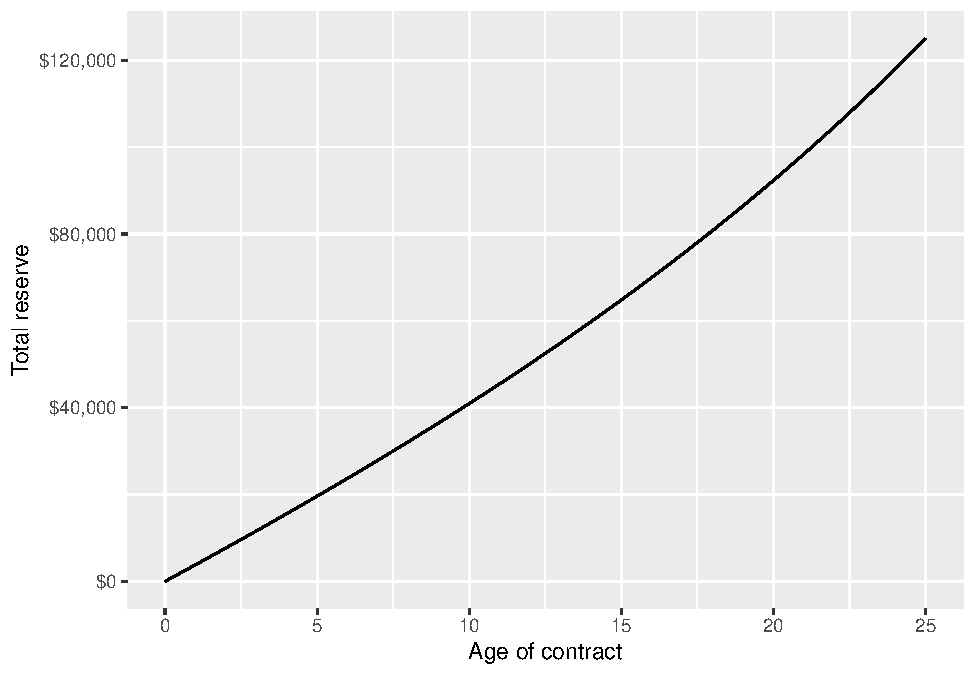
\includegraphics{Exercises-chp_4_files/figure-latex/unnamed-chunk-12-1.pdf}

\end{document}
